%\chapter{Introduction}
%already present in the main file

\graphicspath{{../img/ch10/}}


Four separate topics are presented in the present thesis and the discipline of Information Extraction is the central point of them. Each topic represents one particular aspect of the Information Extraction discipline.

The first two topics are focused on our original information extraction method based on deep language parsing. The first topic describes how deep language parsing was used in our method in combination with manually designed extraction rules.

The second topic provides an extension of our extraction method by machine learning. We have developed an inductive procedure based on Inductive Logic Programming, which allows automated learning of extraction rules from a learning collection.

The idea of the Semantic Web was the strongest motivation of our research from the very beginning. We wanted to exploit information extraction techniques to speed up the semantic web evolution. The third topic of the thesis presents even more than that. The core of the extraction method was experimentally reimplemented using semantic web technologies. Therefore not only the result of information extraction but also the extraction procedure itself is realized using semantic web technologies. The main advantage of this approach is the possibility to save the extraction rules in so called shareable extraction ontologies.

The last topic of this thesis is the most distant from the original information extraction topic. We have included it because it represents an important part of our research and considerable effort was spent on it. The topic deals with document classification and fuzzy logic. We are investigating the possibility of using information obtained by information extraction techniques to document classification. Our implementation of so called Fuzzy ILP Classifier was experimentally used for the purpose of document classification.

\section{Motivation for Our Extraction Methods}

The main motivation for creating both these methods was an attempt to use deep linguistic analysis of natural language texts. Especially for the Czech language with free word order this seemed reasonable. It is much more straightforward to design extraction rules on the basis of linguistic dependency trees than to struggle with the surface structure of text. In a dependency tree a position of a word is determined by its syntactic (analytical trees) or even semantic role (tectogrammatical trees). So the extraction rules might not be dramatically affected by minor variations of the word order.


\begin{figure}
\centerline{\framebox{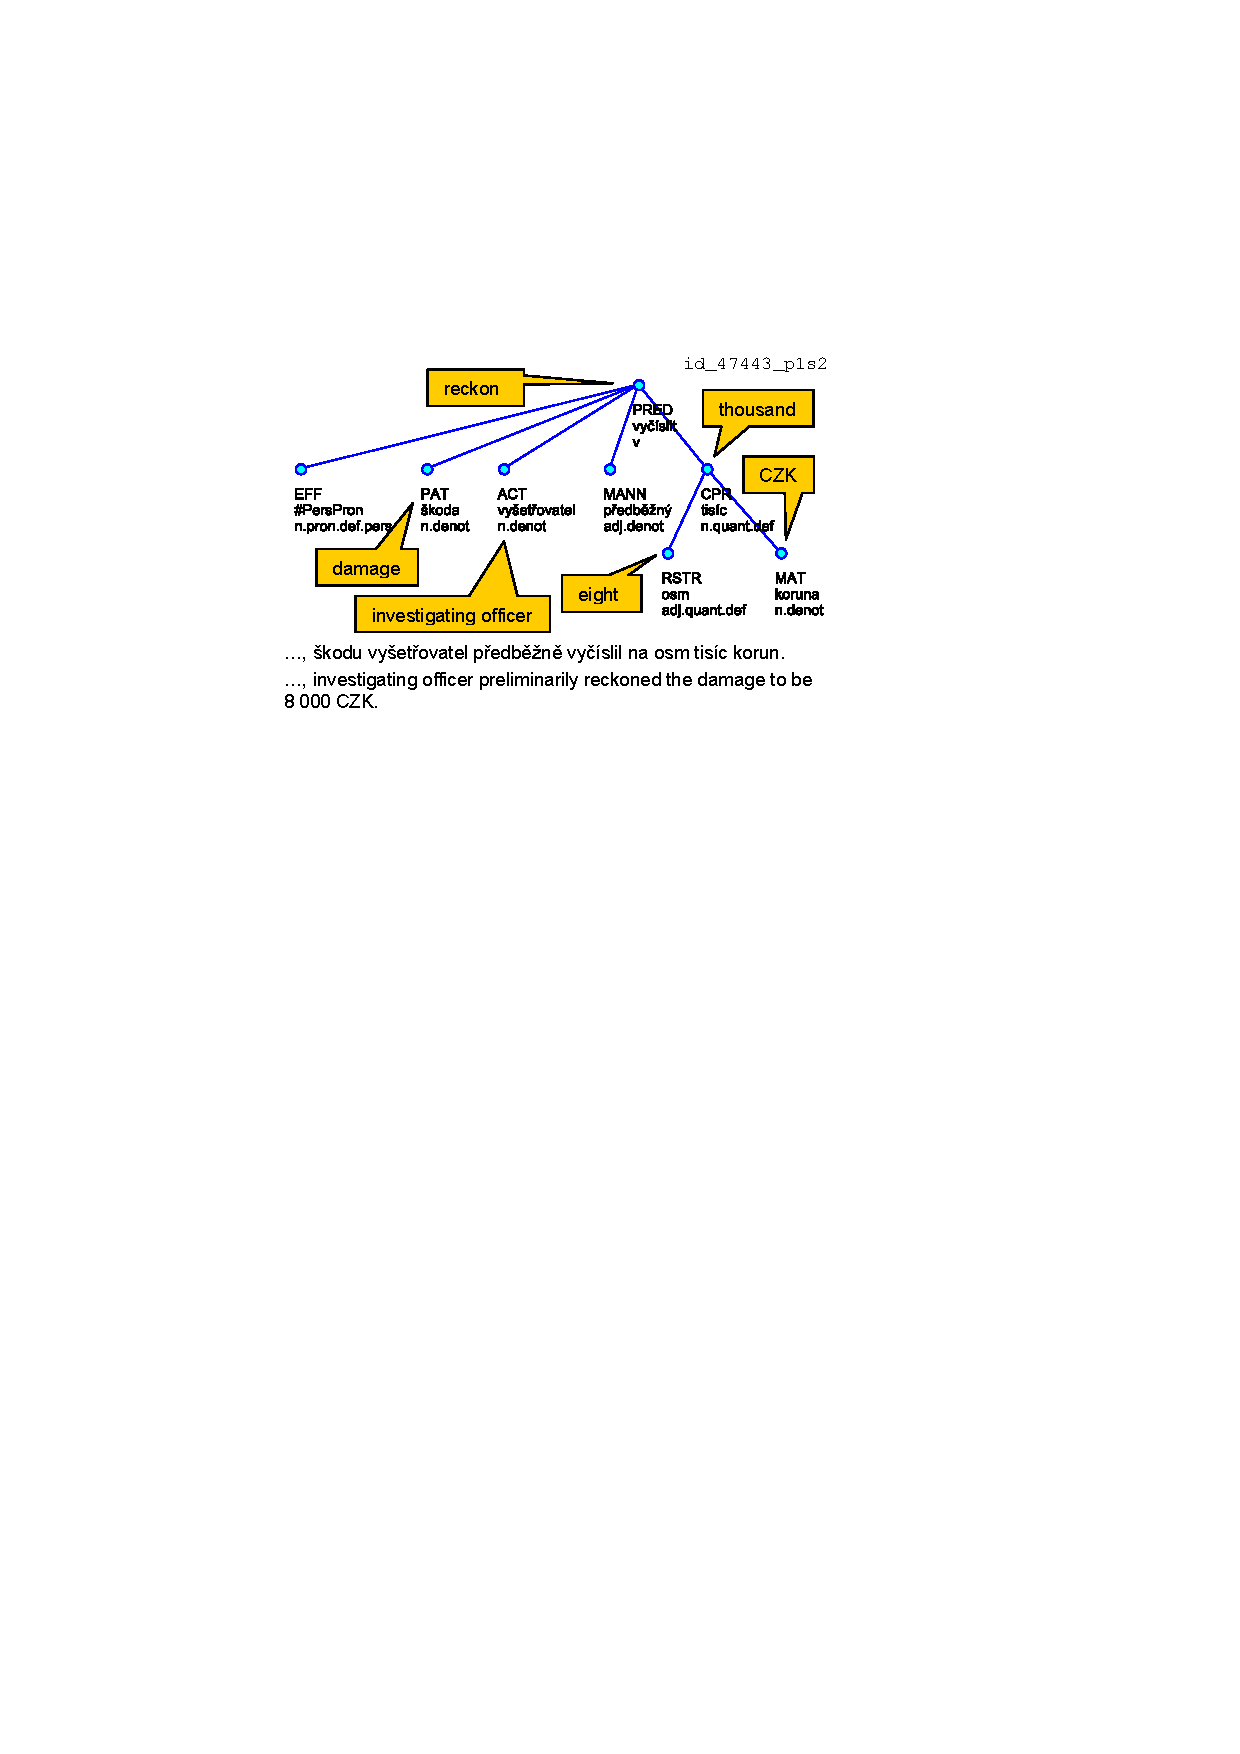
\includegraphics[width=0.55\hsize]{damage_tree}}}
\caption{Example of a linguistic tree of one analyzed sentence.}
\label{fig:intro_damage_tree} 
\end{figure}



\section{Main Goals and Contributions}

To be written!!!

----

The main \emph{contributions} presented in this chapter are \emph{formal models}, prototype \emph{implementation} and experimental \emph{evaluation} of the Fuzzy ILP Classifier.



\section{Organization}

Rather than presenting individual topics or approaches of this thesis separately in distinct chapters, we decided to organize this document according to common aspects of these approaches and to dedicate individual chapters to these aspects instead of individual approaches. This way, all the (four) approaches are described in parallel in each chapter. 

Chapter~\ref{sec:ch_problems} provides definitions of the individual problems and consequent tasks solved in this thesis.

Chapter~\ref{sec:ch_related} contains description of the most related work of other scientists.

Chapter~\ref{sec:ch_third_party} introduces the most important third party tools and resources that were used in our research.

Chapter~\ref{sec:ch_methods} describes solutions, used models and methods if the individual approaches of the present thesis.

Chapter~\ref{sec:ch_implementation} provides details about implementation of all the approaches.

Chapter~\ref{sec:ch_data} describes all datasets that were used in our experiments.

Chapter~\ref{sec:ch_eval} describes all experiments that we performed mostly for evaluation of the approaches.

Chapter~\ref{sec:ch_conclusion} concludes the thesis.

